\documentclass[12pt, a4papre]{article}
\usepackage[catalan]{babel}
\usepackage[unicode]{hyperref}
\usepackage{amsmath}
\usepackage{amssymb}
\usepackage{amsthm}
\usepackage{xifthen}
\usepackage[scientific-notation=true]{siunitx}
\usepackage{xcolor}
\usepackage{listings}
\usepackage{setspace}
\usepackage{graphicx}
\usepackage{circuitikz}
\usepackage{verbatimbox}
\graphicspath{ {/Users/jordivilardell/Desktop/Entregables/Codis/Fotos/} }
\definecolor{mygreen}{rgb}{0,0.6,0}
\definecolor{mygray}{rgb}{0.5,0.5,0.5}
\definecolor{mymauve}{rgb}{0.58,0,0.82}
\definecolor{myorange}{rgb}{0.855,0.576,0.027}
\newcommand\bjtname[1]{($(#1.C)!0.5!(#1.E)$) node[anchor=west]{\killdepth{#1}} }
\lstset{
language=Octave,
frame=single,   
morecomment = [l][\itshape\color{blue}]{\%},
keywordstyle=\color{blue},
commentstyle=\color{mygreen},
breakatwhitespace=false,         
breaklines=true,  
numbers=left,
numbersep=5pt,
numberstyle=\tiny\color{mygray}, 
showstringspaces=false,
showtabs=false,                  
tabsize=2,
stringstyle=\color{myorange},
title=\lstname,
literate=
{+}{{{\color{red}+}}}1
{-}{{{\color{red}-}}}1
{*}{{{\color{red}*}}}1
{,}{{{\color{red},}}}1
{=}{{{\color{red}=}}}1
{;}{{{\color{red};}}}1
{:}{{{\color{red}:}}}1
{[}{{{\color{red}[}}}1
{]}{{{\color{red}]}}}1
{>}{{{\color{red}>}}}1
}

%%%% Dibuixos TikZ
\usepackage{tikz}
\usetikzlibrary{shapes.geometric,calc,arrows.meta,patterns}
% Definicions pels diagrames de blocs
\tikzset{%
  block/.style    = {draw, thick, rectangle, minimum height = 2em,
    minimum width = 3em},
  gain/.style     = {draw, thick, isosceles triangle, minimum height = 2em,
    isosceles triangle apex angle=60},
  port/.style     = {inner sep=0pt, font=\footnotesize},
  sum/.style n args = {4}{draw, circle, node distance = 2cm, minimum size=5mm, alias=sum,
    append after command={
        node at (sum.north) [port, below=1pt] {$#1$}
        node at (sum.west) [port, right=1pt] {$#2$}
        node at (sum.south) [port, above=1pt] {$#3$}
        node at (sum.east) [port, left=1pt] {$#4$}
    },
  }, % Adder
  joint/.style    = {circle, draw, fill, inner sep=0pt, minimum size=3pt},
  input/.style    = {coordinate}, % Input
  output/.style   = {coordinate} % Output
}
% Extensió del tikz per dibuixar dimensions
\usepackage{tikz-dimline}
\newcommand{\norm}[1]{\lvert #1 \rvert}

\hypersetup{
    colorlinks = true,
    linkcolor = blue
}

\author{}
\title{Entregable Circuits i Sistemes Lineals}
\date{}

\begin{document}
	\maketitle
	\textbf{(a)} Per tal de dibuixar la plantilla hem de trobar els seus elements característics:
	\begin{itemize}
	\item freqüència de tall a la que l'amplificació serà de $\frac{1}{\sqrt{2}}$: $2kH$
	\item freqüència amb fita superior d'atenuació: $20kHz$ amb el guany mínim de $74dB$ de la maxima,
	es a dir amb un guany de $10^{-\frac{74}{20}} \approx 2\cdot10^{-4}$.
	\end{itemize}
	I per tant, considerant aquestes dades la plantilla ens quedaria així:
	%Dibuix patró
	\usetikzlibrary{patterns}
	\begin{center}
		\begin{tikzpicture}[scale=2,baseline={(origen.base)}]
			\pgfmathsetmacro{\Hp}{1}
			\pgfmathsetmacro{\Ha}{0.2}
			\pgfmathsetmacro{\Hgap}{0.2}
			\pgfmathsetmacro{\fp}{0.8}
			\pgfmathsetmacro{\fa}{1.3}
			\pgfmathsetmacro{\fb}{2.5}
			% Origen
 			\node (origen) at (0,0) {};
			% Eix X
			\draw[-latex] (-0.1,0) node[left=-2pt] {$0$} -- (2.6,0) node[right=-3pt] {$f[kHz]$};
			% Eix Y
			\draw[-latex] (0,-0.1) node[below=-2pt] {$0$} -- (0,1.5) node[anchor=west] {$|H(\num{j}2\pi\!f)|$};
			% Dimensió Rp
			\dimline[%
				line style={arrows=dimline-dimline},
				label style={font=\scriptsize,right=0pt,rotate=-90,fill=none},
				extension start length=-1,
				extension end length=-1,
			] {(1.2*\fp,\Hp-\Hgap)}{(1.2*\fp,\Hp)}{$3dB$};
			% Límit inferior banda pas
			\fill[gray!10] (0.1pt,0.1pt) -| (\fp,\Hp-\Hgap) -| cycle;
			\fill[pattern=north east lines] (0,\Hp-\Hgap) -| (\fp,0) -| (\fp-0.1,\Hp-\Hgap-0.1) -| cycle; \draw (0,\Hp-\Hgap) -| (\fp,0);
			\draw (\fp,0.05) -- (\fp,-0.05) node[below=0pt] {$2$};
			% Límit superior
			\fill[gray!10] (0.1pt,\Hp) -- (\fa,\Hp) -- (\fa,\Ha) -- (\fb,\Ha) decorate [decoration={random steps,segment length=3pt,amplitude=1pt}] {|- (0.1pt,\Hp+0.3)} -- cycle;
			\fill[pattern=north east lines] (0.1pt,\Hp) -- (\fa,\Hp) -- (\fa,\Ha) -- (\fb,\Ha) -- (\fb, \Ha+0.1) -- (\fa+0.1,\Ha+0.1) -- (\fa+0.1,\Hp+0.1) -- (0.1pt,\Hp+0.1) -- cycle;% 	(0.1,\Hp+0.3) -- (0.1pt,\Hp+0.3) -- cycle;	
			\draw (0.1pt,\Hp) -- (\fa,\Hp) -- (\fa,\Ha) -- (\fb,\Ha);
			% Etiqueta Hp i tick mark
			\draw (-0.05,\Hp)  node[left=-2pt] {$H_\text{màx}=1$} -- (0.05,\Hp);
			% Etiqueta fa i tick mark
			\draw (\fa,0.05) -- (\fa,-0.05) node[below=0pt] {$20$};
			% Etiqueta Ha i tickmark
			\draw[dashed] (\fa,\Ha) -- (0,\Ha); 	\draw (-0.05,\Ha)  node[left=-2pt] {$2\cdot10^{-4}(-74dB)$} -- (0.05,\Ha);
		\end{tikzpicture}
	\end{center}
	
	\textbf{(b)} Hem aconseguit trobar fàcilment la funció de xarxa d'un filtre passabaixes Butterworth d'ordre 2 amb el següent codi d'Octave.
	\begin{lstlisting}
		pkg load signal
		[num,den] = butter(n, 2e3*2*pi,'s');
		disp(num);
		disp(den);
	\end{lstlisting}
	
	I ens ha donat que la funció és la següent

	\[
		H(s)=\frac{\num{1.58e8}}{s^2 +\num{1.78e4} \cdot s +\num{1.58e8}}
	\]
	\newpage
	\textbf{(c/d)} Per tal d'obtenir les amplificacions dels filtres d'ordre $\in\{1, \hdots , 5\}$ en les freqüències demanades hem programat el següent codi d'Octave.	
	\begin{lstlisting}
		pkg load signal
		output_precision(5)

		disp("Tipo Butterworth")
		for n = 1:5
			[num,den] = butter(n,2e3*2*pi,'s');
			H = tf(num,den);
			[mag,fas,w] = bode(H, [0,2e3*2*pi,20e3*2*pi]);
			disp(n);
			disp(mag)
		end
	\end{lstlisting}
	
	I ens ha permès completar la següent taula
	\begin{center}
		\begin{tabular}{ |c | c  c  c|}
			\hline
			Ordre & Amplificació a 0Hz	& Amplificació a 2kHz 	& Amplificació a 20kHz \\ \hline
			1 &1 		 				& 0.707  				& $10^{-1}	$		\\ 
			2 &1 						& 0.707				& $10^{-2}	$		\\
			3 &1 						& 0.707				& $10^{-3}	$		\\
			4 &1 						& 0.707				& $10^{-4}	$		\\
			5 &1 						& 0.707				& $10^{-5}	$		\\
			\hline
		\end{tabular}
	\end{center}
	
	\textbf{(e)} Seguint el mateix procediment comentat anteriorment i amb el següent codi obtenim la funció de xarxa del filtre de Txebixov tipus 1
	\begin{lstlisting}
		pkg load signal
		[num,den] = cheby1(n, 2e3*2*pi,'s');
		disp(num);
		disp(den);
	\end{lstlisting}
	
	I ens mostra que la funció de xarxa per a $n=2$ és

	\[
		H(s)=\frac{\num{7.91e7}}{s^2 +\num{8.1e3} \cdot s +\num{1.12e6}}
	\]
	
	Obtenim les amplificacions amb un codi semblant a l'anterior
	\begin{lstlisting}
		pkg load signal
		output_precision(5)

		disp("Tipo Txebixoc")
		for n = 1:5
  			[num,den] = cheby1(n,3,2e3*2*pi,'s');
  			H=tf(num,den);
  			[mag,fas,w]=bode(H,[0, 2e3*2*pi,20e3*2*pi]);
  			disp(n);
  			disp(mag);
		end
	\end{lstlisting}
	
	I ens dona la següent taula
	
	\begin{center}
		\begin{tabular}{ |c | c  c  c|}
			\hline
			Ordre & Amplificació a 0Hz	& Amplificació a 2kHz 	& Amplificació a 20kHz \\ \hline
			1 &1 		 				& 0.708  				& $0.1	$		\\ 
			2 &0.708 					& 0.708				& $0.005	$		\\
			3 &1 						& 0.708				& $0.00025$		\\
			4 &0.708					& 0.708				& $1.26\cdot10^{-5}$	\\
			5 &1 						& 0.708				& $6.34\cdot10^{-7}$\\
			\hline
		\end{tabular}
	\end{center}

	\textbf{(f)} Com podem veure clarament a les taules anteriors les amplificacions a 20kHz son inferiors per tot ordre en el filtre de tipus Txebixoc.
	Tot i això els dos filtres tenen un guany inferior al demanat, -74dB o una amplificació inferior a la de 0.0002 a partir de l'ordre 4. Les altres especificacions, 
	és a dir, que tingui una amplificació de $\frac{1}{\sqrt{2}}$ als 2kHz es compleix per tots els ordres, ja que així ho hem imposat al codi 
	i finalment el guany a 0Hz és de 0 sempre per la mateixa raó.
	
	\textbf{(g)} Per a fer aquest apartat he creat un nou codi de Octave en el que primer creo un vector fe freqüències f entre 1Hz i 100kHz amb escalat logarítmic entre mostres.
	Despres he trobat la funció de xarxa i a partir del mètode bode d'Octave he anat aplicant la formula per a trobar l'amplificació en dB en funció de la freqüència a mesura que
	recorria el vector creat anteriorment.
	
	Això ho he fet tant pel primer cas amb el filtre tipus Butterworth com el segon amb el filtre tipus Txebixoc i després he guardat els resultats en un fitxer dades.dat des de el que he
	representat a Grace. El codi d'Octave és el següent:
	
	\begin{lstlisting}
		pkg load signal
		output_precision(5)

		f=logspace(1,5,200)';
		disp(size(f,1))

		[num,den]=butter(4,2e3*2*pi,'s');
		H1=tf(num,den);
		[mag,fas,w]=bode(H1,[0,2e3*2*pi,20e3*2*pi]);

		[num,den]=cheby1(4,3,2e3*2*pi,'s');
		H2=tf(num,den);
		[mag,fas,w]=bode(H2,[0,2e3*2*pi,20e3*2*pi]);

		h1=[]
		for i = 1:size(f,1)
  			h1 = vertcat(h1, 20*log10(bode(H1,f(i)*2*pi)));
		end

		h2=[]
		for i = 1:size(f,1)
  			h2 = vertcat(h2, 20*log10(bode(H2,f(i)*2*pi)));
		end

		aux = [f h1 h2];
		save -ascii dades.dat aux
	\end{lstlisting}
	
	I el grafic que ens ha donat grace es el següent
	\begin{figure}[t]
		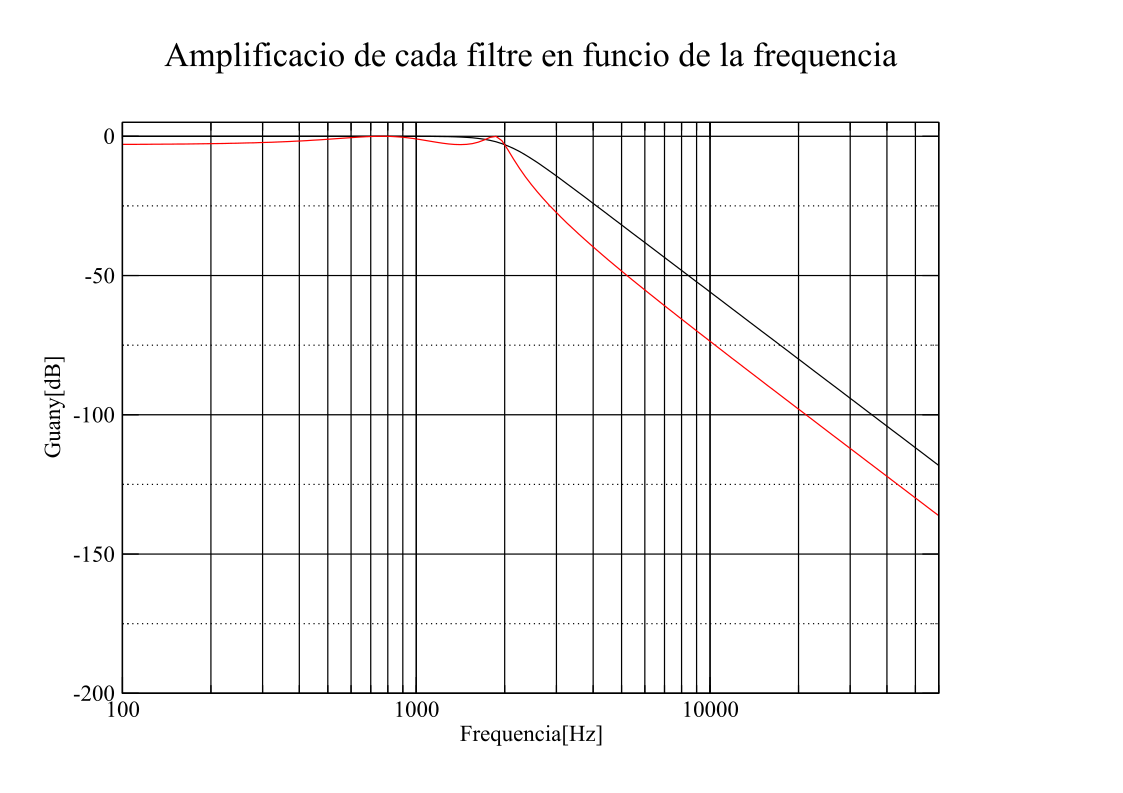
\includegraphics[scale=0.5, angle=0]{GraficaBona.png}	
		\caption{Grafica}
		\label{fig: label}
	\end{figure}
	\newpage
	
	Es pot veure clarament que tant el guany del filtre de Butterworth com la del filtre de Txebixov en la freqüència de 20kHz té una amplificació
	inferior a la demanada, és a dir -74dB
	
	\textbf{(g)} La funció de xarxa de un filtre de tipus Txebixoc de quart ordre es la següent
	
	\[
		H(s)=\frac{\num{3.12e15}}{s^4+\num{7.3e3}\cdot s^3+\num{1.85e8}\cdot s^2 +\num{8.03e11} \cdot s +\num{4.41e15}}
	\]
	
	El circuit que s'usarà per a implementar el filtre és el següent
	
	\begin{center}
		\begin{figure}
		\scalebox{0.85}{
		\begin{circuitikz} 
			\node [op amp,yscale=-1](A1){\texttt{}};
 			\draw (A1.+) to ++(-0.6,0)coordinate(tmp4) to[R=$R_2$] ++(-2,0)coordinate(tmp3)  to[short] ++(0,2) coordinate(tmp) to[C, l_=$C_2$, invert] (tmp -| A1.out) to[short] (A1.out);	
			\draw (A1.-) to [short] ++(0,-1)coordinate(tmp2) to (tmp2 -| A1.out) to[short] (A1.out);
			\draw (tmp3) to [R=$R_1$] ++(-2,0) coordinate(tmp) to[sV, l=$v_{in}$] ++(0,-2.5)node[ground](GND){}coordinate(tmp2);	
			\draw (tmp4) to [C, l_=$C_1$, invert] ++(0,-2.5)node[ground](GND){};
			\draw (A1.out)(1,0)coordinate(tmp5);
			
			\draw (7.5,-0.5)  node [op amp,yscale=-1](A2){\texttt{}};
 			\draw (A2.+) to ++(-0.6,0)coordinate(tmp4) to[R=$R_4$] ++(-2,0)coordinate(tmp3)  to[short] ++(0,2) coordinate(tmp) to[C, l_=$C_4$, invert] (tmp -| A2.out) to[short] (A2.out);	
			\draw (A2.-) to [short] ++(0,-1)coordinate(tmp2) to (tmp2 -| A2.out) to[short] (A2.out);
			\draw (tmp3) to [R=$R_3$] ++(-2,0) coordinate(tmp) to (tmp5);
			\draw (tmp4) to [C, l_=$C_3$, invert] ++(0,-2.5)node[ground](GND){};
			\draw (A2.out) to[short, -o] ++(1,0) node[above](vo){$v_o$};
		\end{circuitikz}
		}
		\end{figure}
	\end{center}
	\newpage
	Com que el circuit de la dreta i el de l'esquerra són iguals podem analitzar-los per separat. La sortida del circuit de l'esquerra ens donarà l'entrada del de la dreta i per tant com que en aquest
	cas no hi ha efecte de càrrega $H_1(s)=\frac{V_i}{V_{o1}}$, $H_2(s)=\frac{V_{o1}}{V_o}$ i per tant
	
	\[
		H(s)=\frac{V_i}{V_o}=\frac{V_i}{V_{o1}}\frac{V_{o1}}{V_o}=H_1(s)H_2(s)
	\]
	
	Així doncs només ens caldrà calcular la $H(S)$ del primer cirquit, ja que el segon té la mateixa canviant els valors de $R_1,R_2,C_1,C_2$ pels respectius $R_3,R_4,C_3,C_4$. Quan tinguem
	les dues fent el producte entre elles arribarem a la $H(s)$ buscada.
	
	Busquem la $H_1(S)$ aplicant KCL als nodes 1 i 2.
	\begin{center}
		\begin{circuitikz} 
			\node [op amp,yscale=-1](A1){\texttt{}};
 			\draw (A1.+) node[label={[font=\footnotesize]-10:$$} ,label={[font=\footnotesize \color{blue}]150:$1$}] {}  
			to ++(-0.6,0)coordinate(tmp4) to[R=$R_2$] ++(-2,0)coordinate(tmp3) node[label={[font=\footnotesize]-10:$$} 
			,label={[font=\footnotesize \color{blue}]150:$2$}] {} to[short] ++(0,2) coordinate(tmp) to[C, l_=$C_2$, invert] (tmp -| A1.out) to[short] (A1.out);	
			
			\draw (A1.-) to [short] ++(0,-1)coordinate(tmp2) to (tmp2 -| A1.out) to[short] (A1.out);
			\draw (tmp3) to [R=$R_1$] ++(-2,0) coordinate(tmp) to[sV, l=$v_{in}$] ++(0,-2.5)node[ground](GND){}coordinate(tmp2);	
			\draw (tmp4) to [C, l_=$C_1$, invert] ++(0,-2.5)node[ground](GND){};
			\draw (A1.out)(1,0)coordinate(tmp5);
			\draw (A1.out) to[short, -o] ++(1,0) node[above](vo){$v_o$};
		\end{circuitikz}
	\end{center}
	\newpage
	Tenint en compte que $V_o=V_2$ obtenim les següents equacions les següents equacions
	
	\begin{equation}
		\frac{V_o-V_1}{R2}+V_oC_1s=0
	\end{equation}
	\begin{equation}
		\frac{V_1-V_i}{R1}+(V_1-V_o)C_2s+\frac{V_1-V_o}{R2}=0
	\end{equation}
	
	De la (1) podem treure que 
	\[
		\frac{V_1}{R_2}=V_o\left(\frac{1}{R_2}+C_1\right)
	\]
	\[
		V_1=V_o\left(C_1R_2s+1\right)
	\]
	I de la (2) 
	
	\[
		V_1\left(\frac{1}{R_1}+C_2s+\frac{1}{R_2}\right)-V_o\left(C_2s+\frac{1}{R_2}\right)=\frac{V_i}{R_1}
	\]
	
	Substituint el resultat obtingut de la (1) en el de la (2) trobem el següent
	
	\[
		V_o\left(\frac{C_1R_2s+1}{R_1}+C_1C_2R_2s^2+C_2s+\frac{C_1R_2s+1}{R_2}-C_2s-\frac{1}{R_2}\right)=\frac{V_i}{R_1}
	\]
	\[
		V_o(C_1(R_1+R_2)s+1+C_1C_2R_1R_2s^2)=V_i
	\]
	\[
		\frac{V_o}{V_i}=\frac{1}{C_1C_2R_1R_2s^2+C_1(R_1+R_2)s+1}
	\]
	\[
		\boxed{H_1(s)=\frac{\frac{1}{C_1C_2R_1R_2}}{s^2+\frac{R_1+R_2}{C_2R_1R_2}s+\frac{1}{C_1C_2R_1R_2}}}
	\]
	
	I per tant la H(s) serà
	
	\[
		\boxed{H(s)=|H(0)|\frac{\frac{1}{C_1C_2R_1R_2}}{s^2+\frac{R_1+R_2}{C_2R_1R_2}s+\frac{1}{C_1C_2R_1R_2}}\cdot
		\frac{\frac{1}{C_3C_4R_3R_4}}{s^2+\frac{R_3+R_4}{C_4R_3R_4}s+\frac{1}{C_3C_4R_3R_4}}}
	\]
	
	Si descomponem amb l'Octave la funció de xarxa mencionada al principi de l'apartat en dues funcions amb el denominador de grau dos obtenim el següent
	
	\[
		H(s)=0.707\cdot\frac{\num{1.42e8}}{s^2+\num{2.14e3}s+\num{1.42e8}} \cdot \frac{\num{3.09e7}}{s^2+\num{5.17e3}s+\num{3.09e7}}
	\]
	
	Ara si ho igualem amb la funció de xarxa que hem tret del circuit veiem que
	
	\[
		|H(0)|=0.707
	\]
	\[
		H_1(s)=\frac{\frac{1}{C_1C_2R_1R_2}}{s^2+\frac{R_1+R_2}{C_2R_1R_2}s+\frac{1}{C_1C_2R_1R_2}}=
		\frac{\num{1.42e8}}{s^2+\num{2.14e3}s+\num{1.42e8}}
	\]
	\[
		H_2(s)=\frac{\frac{1}{C_3C_4R_3R_4}}{s^2+\frac{R_3+R_4}{C_4R_3R_4}s+\frac{1}{C_3C_4R_3R_4}}=
		\frac{\num{3.09e7}}{s^2+\num{5.17e3}+\num{3.09e7}}
	\]
	
	És a dir, dos sistemes de quatre variables d'on es poden treure dues equacions, per tant haurem d'assignar abans els valors de dos components. Imposem que
	$R_1=R_2=10\si{k\ohm}$. Ara busquem quan val $C_1$ i $C_2$.
	
	\[
		2140=\frac{R_1+R_2}{C_2R_1R_2}=\frac{\num{20e3}}{C_210^8} \iff C_2=\frac{\num{20e3}}{\num{2140e8}}=93.45nF
	\]
	
	\[
		\num{1.42e8}=\frac{1}{C_1C_2R_1R_2}=\frac{1}{93.46C_1} \iff C_1=\frac{1}{\num{1.42e8}\cdot93.46}=753.5pF
	\]
	
	Anàlogament trobem el valors de $C_3$ i $C_4$ imposant que $R_3=R_4=10\si{k\ohm}$
	
	\[
		5170=\frac{R_3+R_4}{C_4R_3R_4}=\frac{\num{20e3}}{C_210^8} \iff C_4=\frac{\num{20e3}}{\num{5170e8}}=38.68nF
	\]
	
	\[
		\num{3.09e7}=\frac{1}{C_3C_4R_3R_4}=\frac{1}{3.87C_1} \iff C_3=\frac{1}{\num{3.09e7}\cdot3.87}=8.37nF
	\]
	
	I per tant

	\begin{equation} \label{eq1}
	\boxed{
	\begin{array}{rcl}
		R_1=R_2&=R_3=&R_4=10\si{k\ohm} \\
		C_1 & =& 753.5pF \\
		C_2 & =& 93.45nF \\
		C_3 & = &8.37nF \\
		C_4 & = &38.68nF \\
	\end{array}
	}
	\end{equation}
	
	Finalment cal mencionar que perquè es compleixi la primera de les tres equacions mencionades cal posar un divisor de tensió a la sortida.
	Aquest tindrà valors de resistència petits per a evitar l'efecte de càrrega, assignem per tant a $R_b$ el valor de $10\si{\ohm}$ i $R_a$ el calculem
	a partir de l'equació.
		
	\[
		\frac{10}{10+R_a}=\frac{1}{\sqrt{2}} \iff R_a=4.142\si{\ohm}
	\]
	
	\begin{center}
		\begin{figure}
		\scalebox{0.76}{
		\begin{circuitikz} 
			\node [op amp,yscale=-1](A1){\texttt{}};
 			\draw (A1.+) to ++(-0.6,0)coordinate(tmp4) to[R=$R_2$] ++(-2,0)coordinate(tmp3)  to[short] ++(0,2) coordinate(tmp) to[C, l_=$C_2$, invert] (tmp -| A1.out) to[short] (A1.out);	
			\draw (A1.-) to [short] ++(0,-1)coordinate(tmp2) to (tmp2 -| A1.out) to[short] (A1.out);
			\draw (tmp3) to [R=$R_1$] ++(-2,0) coordinate(tmp) to[sV, l=$v_{in}$] ++(0,-2.5)node[ground](GND){}coordinate(tmp2);	
			\draw (tmp4) to [C, l_=$C_1$, invert] ++(0,-2.5)node[ground](GND){};
			\draw (A1.out)(1,0)coordinate(tmp5);
			
			\draw (7.5,-0.5)  node [op amp,yscale=-1](A2){\texttt{}};
 			\draw (A2.+) to ++(-0.6,0)coordinate(tmp4) to[R=$R_4$] ++(-2,0)coordinate(tmp3)  to[short] ++(0,2) coordinate(tmp) to[C, l_=$C_4$, invert] (tmp -| A2.out) to[short] (A2.out);	
			\draw (A2.-) to [short] ++(0,-1)coordinate(tmp2) to (tmp2 -| A2.out) to[short] (A2.out);
			\draw (tmp3) to [R=$R_3$] ++(-2,0) coordinate(tmp) to (tmp5);
			\draw (tmp4) to [C, l_=$C_3$, invert] ++(0,-2.5)node[ground](GND){};
			\draw (A2.out) to[R=$R_a$] ++(2,0)coordinate(tmp) to[short, -o] ++(0.5,0) node[above](vo){$v_o$};
			\draw (tmp) to [R=$R_b$] ++(0,-2)node[ground](GND){};
		\end{circuitikz}
		}
		\end{figure}
	\end{center}
	\newpage
	\textbf{(h)} Finalment fem la simulació amb el Gnucap. El codi programat és el següent
	
	\begin{lstlisting}
		.INCLUDE uA741.ckt

		Vcc+ 8 0 DC 100
		Vcc- 9 0 DC -100
		
		Vi 10 0 ac 1 phase=0
		Ra 10 1 4.1421
		Rb 1 0 10
	
		R1 1 2 10k
		R2 2 3 10k
		C1 3 0 753.5p
		C2 2 4 93.45n
		X1 3 4 8 9 4 uA741
		
		R3 4 5 10k
		R4 5 6 10k
		C3 6 0 8.37n
		C4 5 7 38.68n
		X2 6 7 8 9 7 uA741
		
		.print ac vdb(7) 
		.op
		.AC dec 1000 10 100k
		.end
	\end{lstlisting}
	
	I graficant els resultats a Grace hem obtingut la gràfica esperada, mostrada a continuació
	
	\begin{figure}[t]
		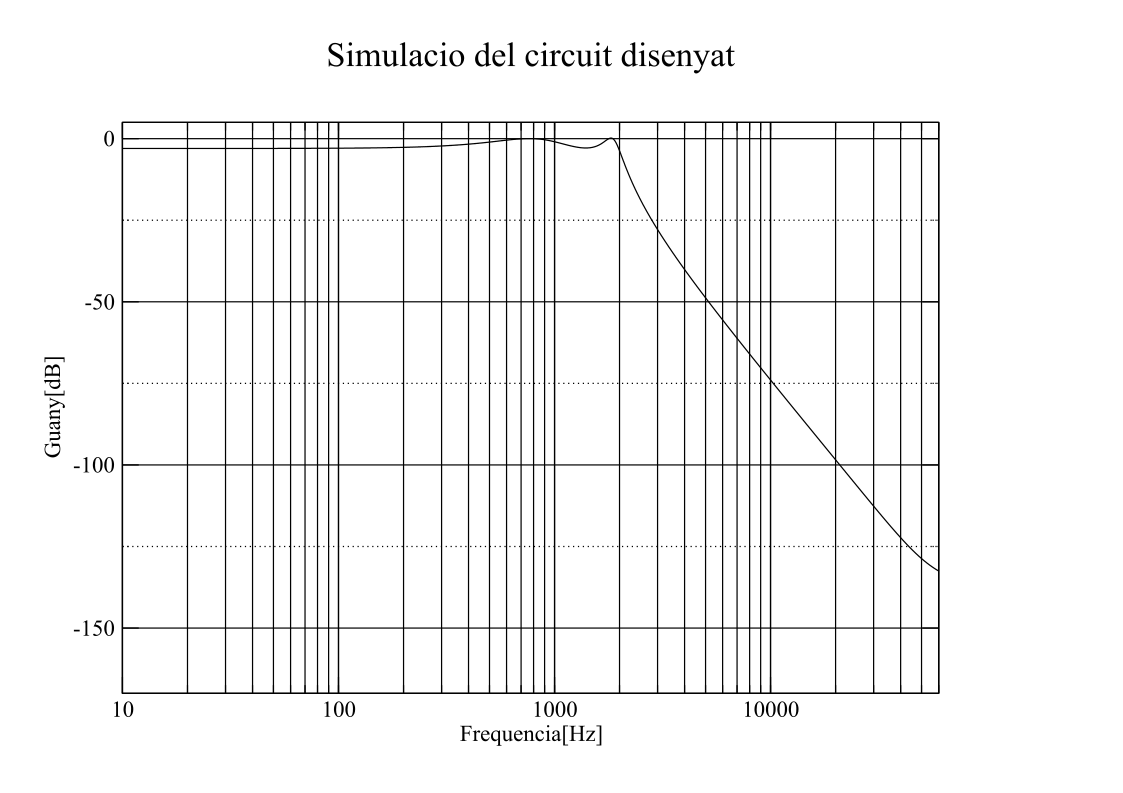
\includegraphics[scale=0.5, angle=0]{GraficaSimBona.png}	
		\caption{Grafica de la simulació}
		\label{fig: label}
	\end{figure}
	
\end{document}